\subsubsection*{}

\begin{enumerate}
%%%%%%%%%%%%%%%%
\item Usain Bolt es un atleta jamaicano especialista en pruebas de velocidad, ostenta el record de velocidad por correr $100.0$ m en $10.0$ s, sin embargo el atleta afirma que puede recorrer la misma distancia en $9.4$ s, los analistas están seguros que puede superar sus marcas ya que el atleta baja su ritmo al final de la carrera cuando sabe que ha ganado. ¿Cuál es la velocidad máxima media del atleta? \label{dia-1}

\begin{enumerate}[(A)]
\item $10.0\frac{m}{s}$
\item $10.6\frac{m}{s}$
\item $11.0\frac{m}{s}$
\item $9.4\frac{m}{s}$
\end{enumerate}

%%%%%%%%%%%%%%%%%%%%%
\item Asuma que, para el record, al atleta le toma un segundo acelerar desde el reposo a su velocidad máxima media y faltando $2$ s para finalizar la carrera comienza a desacelerar constantemente. ¿Cuál es la magnitud de esta desaceleración?\label{dia-2}

\begin{enumerate}[(A)]
\item $-5.3 \frac{m}{s^2}$
\item $-5.0 \frac{m}{s^2}$
\item $+5.3 \frac{m}{s^2}$
\item $+5.0 \frac{m}{s^2}$
\end{enumerate}

%%%%%%%%%%%%%%%%%%%%%%%%
\newpage
\item Una gráfica correcta de este movimiento sería: \label{dia-3}\\

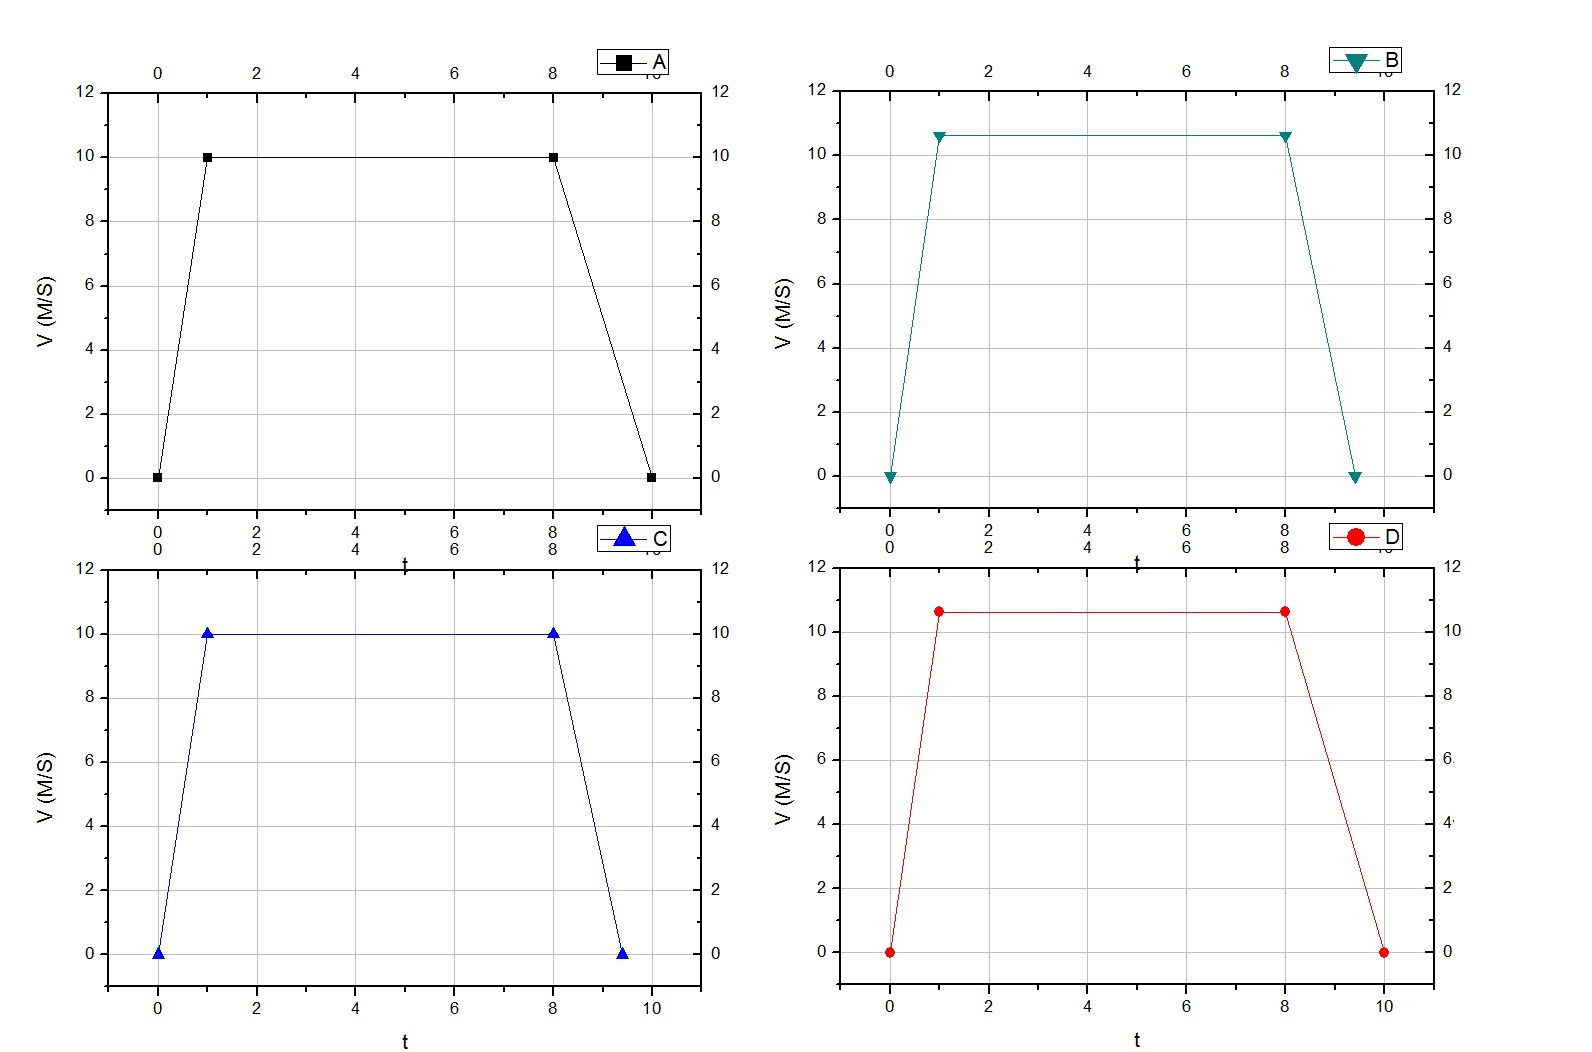
\includegraphics[width=0.45\textwidth]{dia1}


%%%%%%%%%%%%%%%%%%%%%%%%%

\item Supongamos que el atleta compite en un día con mucho viento, imagine que la velocidad del viento es aproximadamente $5.5\frac{m}{s}$, lastimosamente no supera su record y recorre $100$ m en $16$ s. \label{dia-4}
\noindent Una representación correcta con los valores dados en $\frac{m}{s}$ es:

% yo cambie el orden de la numeraciòn que tenia diana es decir cambie la figura llamada 2 y 1 por dia1 y dia2
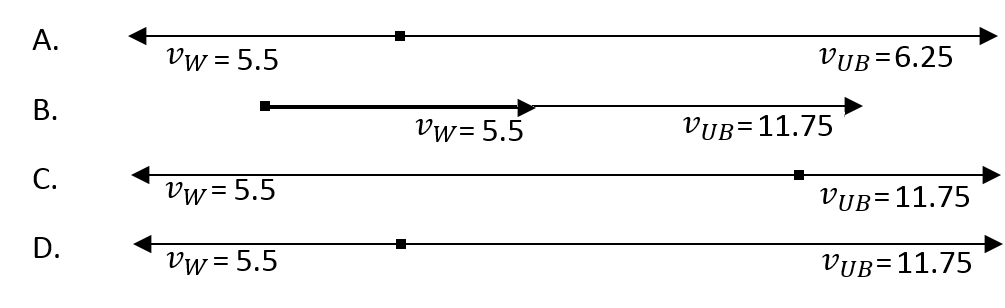
\includegraphics[width=0.45\textwidth]{dia2}

%%%%%%%%%%%%%%%%%%%%%%
\item Teniendo en cuenta lo anterior en un día sin viento, se hubiera superado el record? Justifique su respuesta claramente \label{dia-5} \hrulefill\\
\_\hrulefill\\
\_\hrulefill\\
\_\hrulefill.

%%%%%%%%%%%%%%%%%%%%%
\newpage
\item Thomas Muller, un futbolista alemán se encuentra practicando lanzando penaltis frente al arco de futbol. La distancia reglamentaria para cobrar un penalti es de $11$ m del arco, con un arco de $2.4$ m de altura. \label{dia-6}
\noindent ¿Cuál es la velocidad máxima vertical que debe imprimirle el jugador al balón para que haga gol? (Asuma que el balón tiene energía cinética nula en el eje Y)

\begin{enumerate}[(A)]
\item $4 \sqrt{2}\frac{m}{s}$
\item $4 \sqrt{3}\frac{m}{s}$
\item $4.0\frac{m}{s}$
\item Faltan datos en el problema
\end{enumerate}

%%%%%%%%%%%%%%%%%%%%%%%%%

\item ¿Cuánto tiempo dura el balón en el aire antes de conocer si es gol o no? (Recuerde que $\sqrt{3}>\sqrt{2}$) \label{dia-7}

\begin{enumerate}[(A)]
\item $0.56$ s
\item $0.69$ s
\item $0.40$ s
\item Faltan datos en el problema
\end{enumerate}

%%%%%%%%%%%%%%%%%%%%%%%%
\noindent Un tornamesa es un aparato para reproducir discos de vinilo. Asumamos uno de estos de $45$ RPM con un disco de $12$ pulgadas. 

\begin{center}
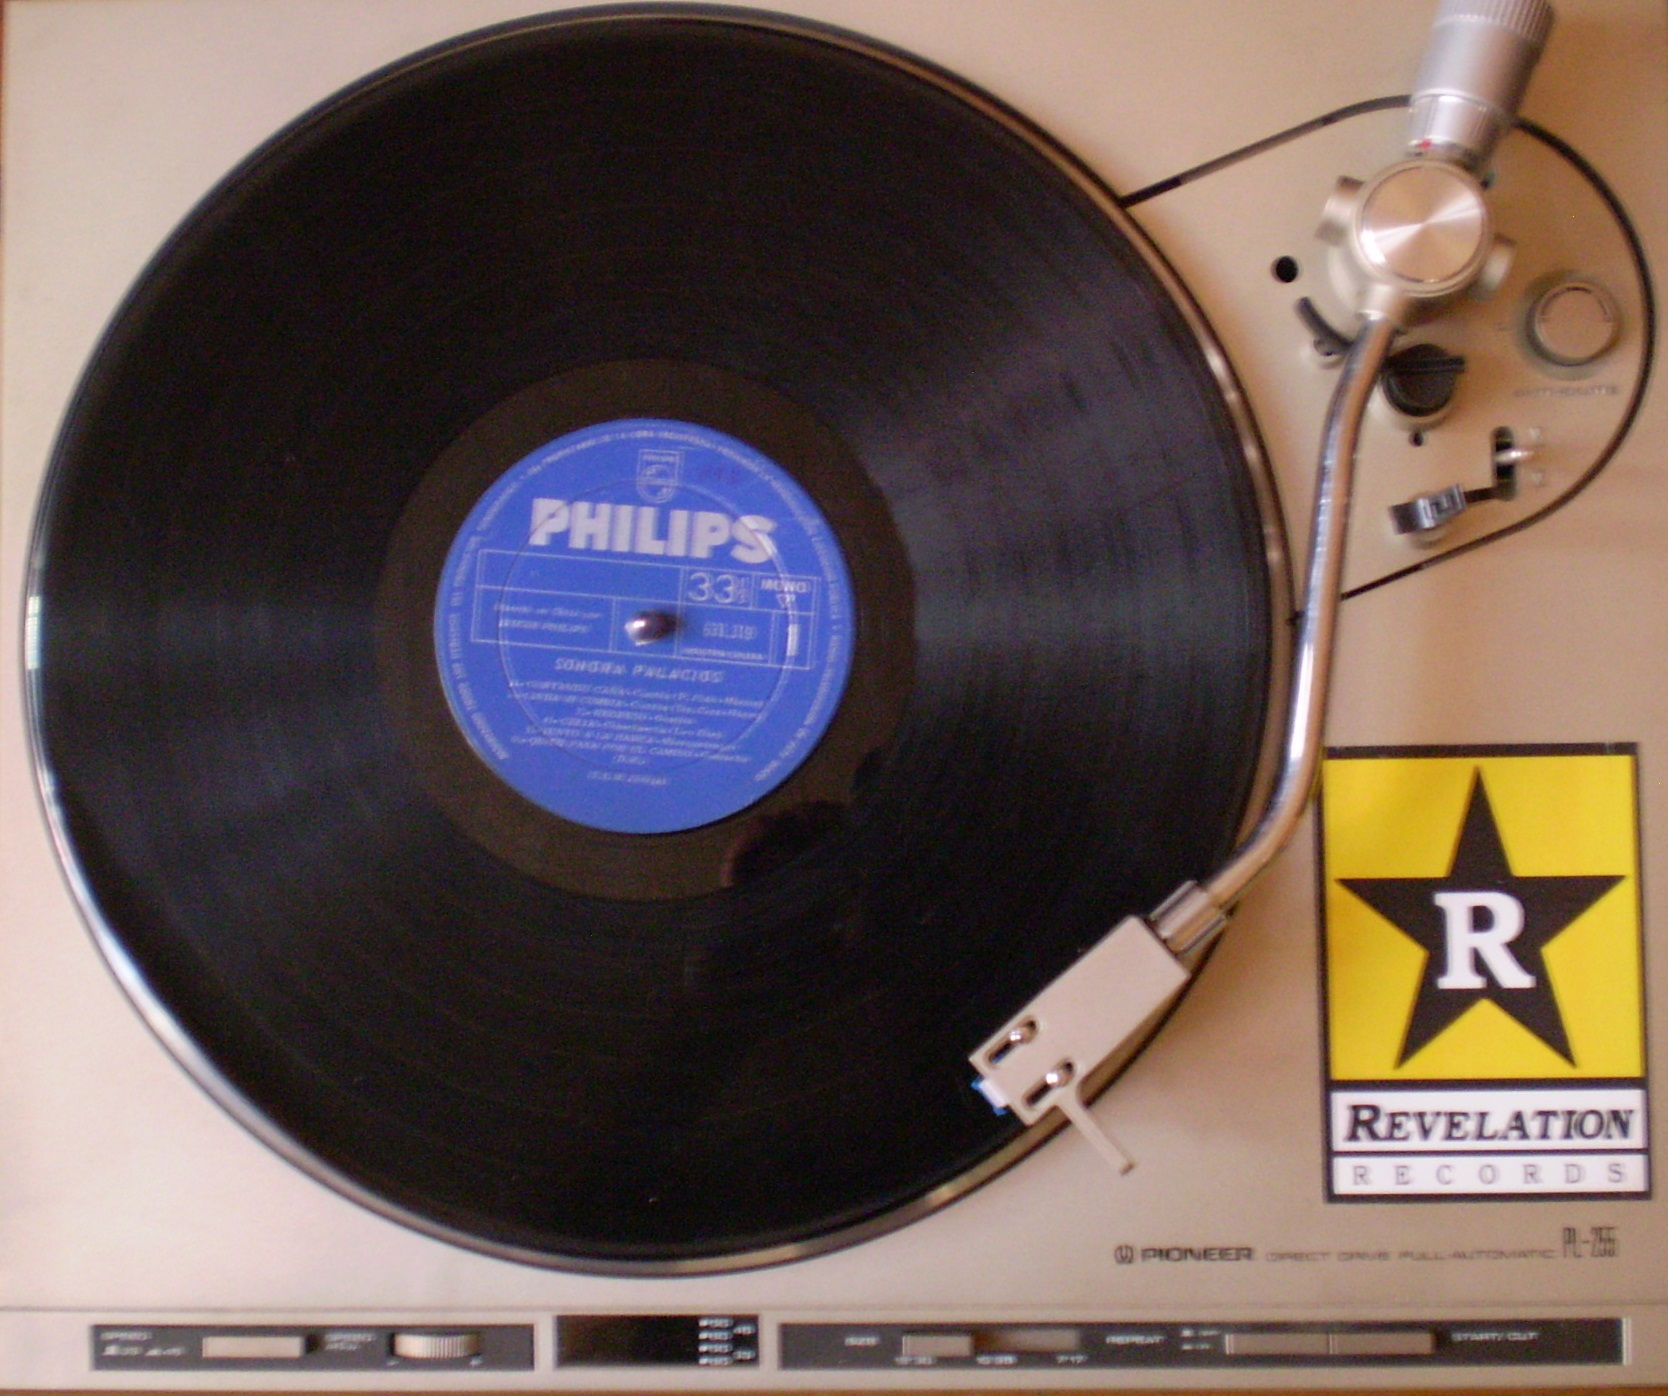
\includegraphics[width=0.35\textwidth]{dia3}
\end{center}

\newpage
\item ¿Cuál es la velocidad lineal de un punto situado en el borde del disco? \label{dia-8}

\begin{enumerate}[(A)]
\item $540\frac{m}{s}$
\item $32400\frac{pulg}{s}$
\item $540\frac{pulg}{s}$
\item $32400\frac{pulg}{min}$
\end{enumerate}

%%%%%%%%%%%%%%%%%%%%%%%

\item ¿Cuál es su aceleración centrípeta?\label{dia-9}

\begin{enumerate}[(A)]
\item $24300\frac{pulg}{s^2}$
\item $24300\frac{m}{s^2}$
\item $24300\frac{pulg}{min^2}$
\item $24300\frac{m}{min^2}$
\end{enumerate}

%%%%%%%%%%%%%%%%%%%%%%%
\item Cuando una esfera de plomo y una de madera de igual radio caen, la resistencia del aire $R$ que actúa sobre cada una de ellas es prácticamente igual. ¿Qu\'e se puede decir sobre las aceleraciones de las esferas?\label{dia-10}

\begin{enumerate}[(A)]
\item La esfera de plomo está más acelerada que la de madera
\item La esfera de plomo está menos acelerada que la de madera
\item Las aceleraciones son iguales
\item La resistencia del aire no cambia para nada el sistema
\end{enumerate}

%%%%%%%%%%%%%%%%%%%%%%%%%
\item En una campaña ecológica realizada se ha notado que si se vierte una gota de aceite de volumen $0.01cm^3$ sobre una piscina esta se expande uniformemente de tal manera que dicha capa tiene un espesor de $10^{-9}m$. ¿Cuál es el área de la piscina de agua contaminada?\label{dia-11}

\begin{enumerate}[(A)]
\item $1m^2$
\item $10m^2$
\item $100m^2$
\item $1000m^2$
\end{enumerate}

%%%%%%%%%%%%%%%%%%%%%%%%%%

\newpage
\item De acuerdo a lo anterior ¿cuántas piscinas de este mismo tamaño se contaminan con un litro de este aceite? \label{dia-12}

\begin{enumerate}[(A)]
\item 1000
\item 10000
\item 100000
\item 1 millon
\end{enumerate}

%%%%%%%%%%%%%%%%%%%%%%%%%
\item ¿Por qué los bomberos tienen que sujetar fuertemente la manguera cuando se lanza agua a alta presión para apagar un incendio? \label{dia-13} \hrulefill\\
\_\hrulefill\\
\_\hrulefill\\
\_\hrulefill.

%%%%%%%%%%%%%%%%%%%%%%%%%%%%

\item Un tubo de crema dental se cierra en la fábrica a la altura de mar y que se lleva un cargamento de estas a Bogotá para su comercialización. Cuando usted compre uno de estos tubos y lo abra la crema dental:\label{dia-14}

\begin{enumerate}[(A)]
\item Saldrá puesto que la presión de empacado es menor que la de sus condiciones actuales
\item Entrará puesto que la presión de empacado es menor que la de sus condiciones actuales
\item Saldrá puesto que la presión de empacado es mayor que la de sus condiciones actuales
\item Entrará puesto que la presión de empacado es mayor que la de sus condiciones actuales
\end{enumerate}

%%%%%%%%%%%%%%%%%%%%%%%%%%%%%
\newpage
\item Se tiene una pelota de $2$ Kg de masa a lo alto de una colina como se muestra en la situación.\label{dia-15}

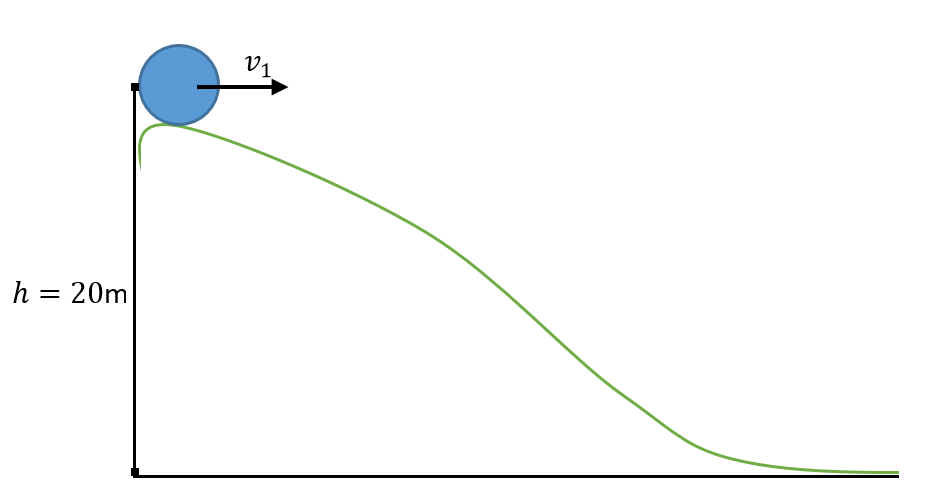
\includegraphics[width=0.45\textwidth]{dia4}

 ¿Cuál es el valor de la energía cinética al llegar al punto más bajo de la rampa? 

\begin{enumerate}[(A)]
\item $mgh$
\item $\frac{1}{2}mgh+\frac{mv_1^2}{2}$
\item $mgh+\frac{mv_1^2}{2}$
\item $mgh+mv_1^2$
\end{enumerate}

%%%%%%%%%%%%%%%%%%%%%%%%%%%%%%%

\item Tome en cuenta lo anterior y asuma que la pelota cae desde lo alto sin ninguna velocidad inicial ¿con qué velocidad llega al punto más bajo? \label{dia-16}

\begin{enumerate}[(A)]
\item $10\sqrt{2}\frac{m}{s}$
\item $20.0\frac{m}{s}$
\item $10.0\frac{m}{s}$
\item $2\sqrt{10}\frac{m}{s}$
\end{enumerate}

%%%%%%%%%%%%%%%%%%%%%%%%%%%%%%%%%%%
\item Una carreta de $20$ Kg se desplaza con una velocidad de $2\frac{m}{s}$. Un instante después una niña de $40$ Kg salta de la carreta con una velocidad en el mismo sentido de la carreta de $1\frac{m}{s}$, la nueva velocidad de la carreta es: \label{dia-17}

\begin{enumerate}[(A)]
\item $2.5\frac{m}{s}$
\item $3.5\frac{m}{s}$
\item $8.0\frac{m}{s}$
\item $4.0\frac{m}{s}$
\end{enumerate}

%%%%%%%%%%%%%%%%%%%%%%%%%%
\newpage
\item Un deposito muy grande de agua sujeto a presión atmosférica tiene un pequeño agujero sobre la pared lateral a una profundidad de $5$ m ¿Cuál es la velocidad de salida del agua? \label{dia-18}

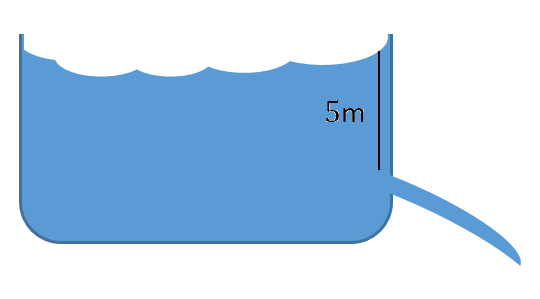
\includegraphics[width=0.45\textwidth]{dia5}

\begin{enumerate}[(A)]
\item $2\sqrt{5}\frac{m}{s}$
\item $5.0\frac{m}{s}$
\item $5\sqrt{2}\frac{m}{s}$
\item $10.0\frac{m}{s}$
\end{enumerate}

%%%%%%%%%%%%%%%%%%%%%%%%%%%%%
\item Un recipiente de $25cm^3$ (mostrado en la figura) contiene un líquido cuya densidad es $1200\frac{Kg}{m^3}$, se sumerge un sólido y $2/5$ partes de él flotan, determine la densidad del sólido. \label{dia-19}

\begin{enumerate}[(A)]
\item $720.0\frac{Kg}{m^3}$
\item $480.0\frac{Kg}{m^3}$
\item $240.0\frac{Kg}{m^3}$
\item No es posible determinarla
\end{enumerate}

%%%%%%%%%%%%%%%%%%%%%%%%%%%%%%
\item En medio de un bosque un leñador ve un relámpago y a los $5$ s escucha el trueno, $30$ s después se encuentra resguardado dentro de la cabaña ¿Cuál es la distancia entre el punto en el que cayó el rayo y la cabaña?\label{dia-20}\\
El sonido viaja aproximadamente a $340\frac{m}{s}$ y la luz a $300000\frac{Km}{s}$. 

\begin{enumerate}[(A)]
\item $10200$ Km
\item $170$ Km
\item $10200$ m
\item $1700$ m
\end{enumerate}


%%%%%%%%%%%%%%%%%%%%%%%%%%%%%%%%%
\item Un resorte con longitud natural $20$ cm, se alarga $5$ cm cuando se ejerce sobre él una fuerza de $2$ N. ¿Cuál es la constante elástica del resorte? \label{dia-21}

\begin{enumerate}[(A)]
\item $0.4\frac{N}{m}$
\item $0.1\frac{N}{m}$
\item $40\frac{N}{m}$
\item $10\frac{N}{m}$
\end{enumerate}

%%%%%%%%%%%%%%%%%%%%%%%%%%%%%%%%%
\item En un juego se tiene que mover una pelota pesada desde el reposo hasta una distancia máxima, uno de los jugadores tira la pelota de $5$ Kg a $25$ m en $5$ s. Asuma que la aceleración es constante, Cuál es la fuerza horizontal que el jugador ejerció sobre la pelota? \label{dia-22}

\begin{enumerate}[(A)]
\item $25$ N
\item $12.5$ N
\item $50$ N
\item $10$ N
\end{enumerate}

%%%%%%%%%%%%%%%%%%%%%%%%%%%%%%%%%
\item En una película de ciencia ficción una nave se encuentra en la mitad entre la Tierra y Marte cuando de repente un misil la golpea y se ve una explosión, un astronauta observando a la distancia puede ver la escena, pero ¿qué ruido siente?\label{dia-23}

\begin{enumerate}[(A)]
\item Ninguno
\item Uno que varía en intensidad dependiendo de la distancia a la cual se sitúe el astronauta
\item Uno idéntico al que se escucharía en la tierra pero más sordo 
\item Uno idéntico al que se escucharía en la tierra 
\end{enumerate}

%%%%%%%%%%%%%%%%%%%%%%%%%%%%%%%%%
\newpage

\item Dos recipientes cilíndricos abiertos en los cuáles se puede medir el nivel contienen el mismo líquido, se unen en la base por un tubo. En el cilindro 1 se vierte agua, como es posible que las medidas en los cilindros sean distintas? \label{dia-24}

\begin{enumerate}[(A)]
\item Inicialmente ambos estaban vacíos
\item Inicialmente contenían agua a distintos niveles
\item Inicialmente contenían un líquido distinto al agua
\item Tenían un diámetro distinto 
\end{enumerate}


%%%%%%%%%%%%%%%%%%%%%%%%%%%%%%%%%
\newpage
\item La luz es un tipo de onda \label{dia-25}
\begin{enumerate}[I.]
\item Transversal
\item Longitudinal
\item Electromagnética
\item Mecánica
\end{enumerate}


\begin{enumerate}[(A)]
\item I y III
\item I y IV
\item II y III
\item II y IV
\end{enumerate}



%%%%%%%%%%%%%%%%%%%%%%%%%%%%%
\end{enumerate}
%%%%%%%%%%%%%%%%%%%%%%%%%%%%%5

